% flashcards-title: Ladder of four length units
% flashcards-desc: Four boxes in a row from smallest to largest unit: millimeter, centimeter, meter, kilometer. Between neighboring boxes, connectors state the exact relations: one centimeter equals ten millimeters, one meter equals one hundred centimeters, and one kilometer equals one thousand meters. Arrows note that units grow toward the right and shrink toward the left.
\documentclass[dvisvgm,tikz,border=8pt]{standalone}
\usepackage{tikz}
\usetikzlibrary{arrows.meta,calc,positioning}
\definecolor{DeckInk}{HTML}{172A3A}
\definecolor{DeckAccent}{HTML}{176B87}
\definecolor{DeckWarm}{HTML}{D97706}
\definecolor{DeckMuted}{HTML}{667784}
\definecolor{DeckPaper}{HTML}{F7FAFC}
\tikzset{
  every node/.style={font=\sffamily, text=DeckInk},
  object/.style={draw=DeckInk, line width=1.1pt, fill=DeckPaper},
  primary/.style={draw=DeckAccent, line width=1.5pt},
  boundary/.style={draw=DeckAccent, line width=1.5pt, dashed, rounded corners=6pt},
  guide/.style={draw=DeckMuted, line width=0.9pt, dashed},
  dimension/.style={{Stealth[length=3.2mm,width=2.2mm]}-{Stealth[length=3.2mm,width=2.2mm]}, draw=DeckWarm, line width=1.2pt},
  motion/.style={-{Stealth[length=3.5mm,width=2.5mm]}, draw=DeckAccent, line width=1.5pt, dashed},
}

\begin{document}
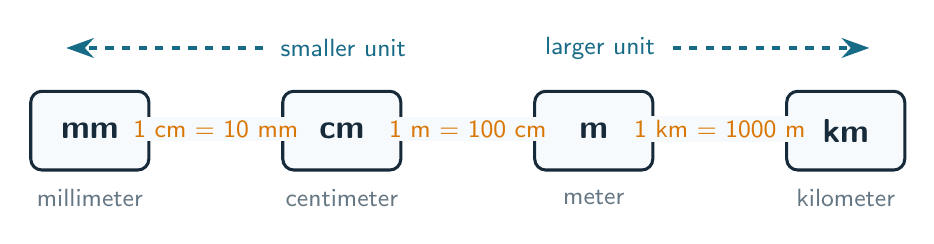
\begin{tikzpicture}[x=1cm,y=1cm]
  % Unit boxes from smallest to largest
  \node[object, rounded corners=4pt, minimum width=1.5cm, minimum height=1.0cm,
        font=\sffamily\bfseries\large] (mm) at (0,0) {mm};
  \node[object, rounded corners=4pt, minimum width=1.5cm, minimum height=1.0cm,
        font=\sffamily\bfseries\large] (cm) at (3.2,0) {cm};
  \node[object, rounded corners=4pt, minimum width=1.5cm, minimum height=1.0cm,
        font=\sffamily\bfseries\large] (m)  at (6.4,0) {m};
  \node[object, rounded corners=4pt, minimum width=1.5cm, minimum height=1.0cm,
        font=\sffamily\bfseries\large] (km) at (9.6,0) {km};

  % Unit names beneath the boxes
  \node[text=DeckMuted, font=\sffamily\small] at (0,-0.85) {millimeter};
  \node[text=DeckMuted, font=\sffamily\small] at (3.2,-0.85) {centimeter};
  \node[text=DeckMuted, font=\sffamily\small] at (6.4,-0.85) {meter};
  \node[text=DeckMuted, font=\sffamily\small] at (9.6,-0.85) {kilometer};

  % Connectors with exact relations
  \draw[guide] (mm) -- (cm);
  \draw[guide] (cm) -- (m);
  \draw[guide] (m) -- (km);
  \node[text=DeckWarm, font=\sffamily\small, fill=DeckPaper, inner sep=1.5pt]
        at (1.6,0.02) {1 cm = 10 mm};
  \node[text=DeckWarm, font=\sffamily\small, fill=DeckPaper, inner sep=1.5pt]
        at (4.8,0.02) {1 m = 100 cm};
  \node[text=DeckWarm, font=\sffamily\small, fill=DeckPaper, inner sep=1.5pt]
        at (8.0,0.02) {1 km = 1000 m};

  % Direction cues, redundant with left-to-right ordering
  \draw[motion] (7.4,1.05) -- (9.9,1.05);
  \node[text=DeckAccent, font=\sffamily\small, anchor=east] at (7.3,1.05) {larger unit};
  \draw[motion] (2.2,1.05) -- (-0.3,1.05);
  \node[text=DeckAccent, font=\sffamily\small, anchor=west] at (2.3,1.05) {smaller unit};
\end{tikzpicture}
\end{document}
